\chapter{Introduction}
Community detection, or graph clustering,  can be informally described as the process of partitioning the vertices of a given graph into non-overlapping groups that are more densely connected internally. Since most network exhibits a community structure \cite{comm_dete_in_graphs}, this problem has a significant impact on numerous real-world applications. For example, in social network, to divide individuals into groups according to the frequency of their interactions \cite{social}, or in protein-protein interaction networks, to identify clusters of proteins that perform identical functions within a cell \cite{bio}. Therefore, this problem has sparked huge interest across different scientific communities, such as network science, social science, bioinformatics, machine learning and statistical physics, since the 1980s. Despite the development of a remarkable variety of models and algorithms, the challenge remains unsolved, as it is a $\mathcal{NP}$-hard problem in general \cite{np-hard}.\\

To address the community detection problem, a rigorous mathematical framework is essential. Although various effective models exist, such as \textit{Markov random field} and \textit{factor graph model}. However, this report adopts a probabilistic generative model, called \textit{stochastic block model (SBM)}, because it is arguably the most representative one due to its canonicality. Moreover, the SBM exhibits a phase transition phenomenon, known as the Kesten-Stigum Bound Conjecture, where community detection is impossible when the Signal-to-Noise Ratio (SNR) is less than one (hard regime), while efficient algorithms exist for SNR greater than one (easy regime) \cite{Emmanuel2023} \cite{deeplearning}.\\

\begin{figure}[h]
    \centering
    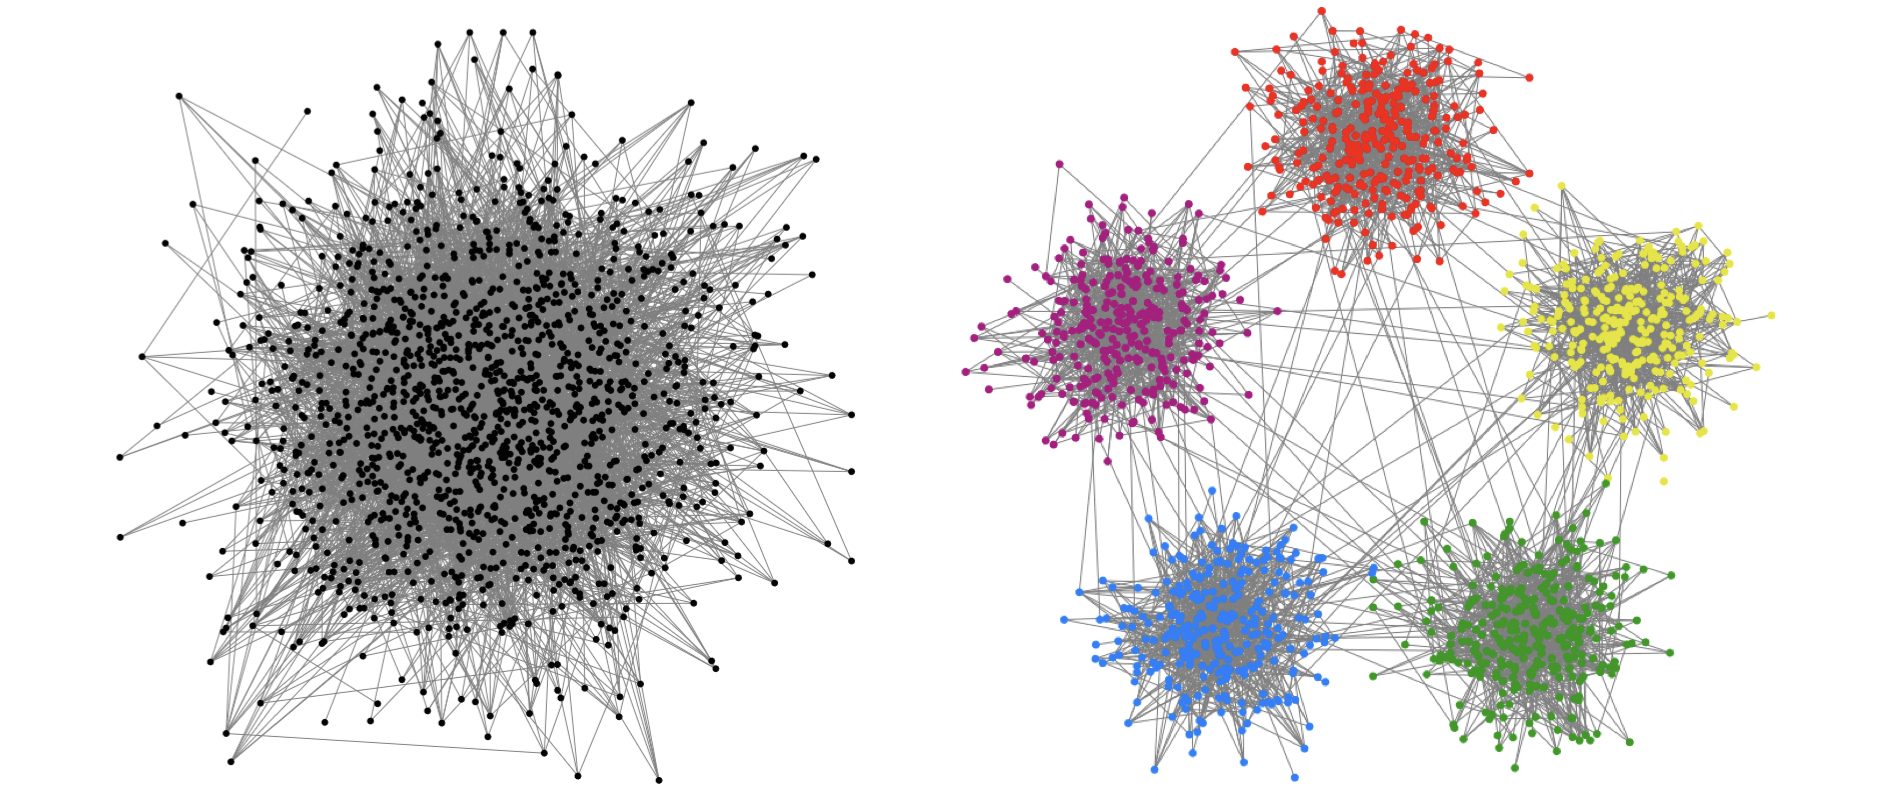
\includegraphics[width=1\linewidth]{Figures/community.jpg}
    \caption[Community Structure]{The left graph is drawn from an SBM with 1000 vertices, 5 built-in communities, vertices inside the same community are connected with probability $1/50,$ and vertices across different communities connected with probability $1/1000.$ This figure is cited from \cite{TheConjecture}. The goal of community detection is to recover the community structure as shown in the right graph from the left graph up to some level of accuracy.}
    \label{fig:community}
\end{figure}

This report will stick closely with the Kesten-Stigum Bound Conjecture, and its structure will be organised based on the SNR value. We will first introduce an existing solution known as the Spectral Algorithm for the easy regime (SNR $>1$). We will then delve into the more challenging hard regime (SNR $\leq1$).\\
The goal of this project is to solve the community detection problem in the hard regime with the aid of additional information, called partial seed set. We propose a greedy recovery algorithm under this setting and discuss some improvements to this algorithm tailored to specific objective conditions, finally extending it to the case of multiple communities.\\

Before proceeding, we will first formally define the problem and introduce some important concepts that will be used throughout this report.

\section{Formal Definition}
\subsection{Key Concepts}
How can we measure the concept of community?  While traditional definitions relied on counting the number of internal and external edges, the modern perspective emphasises the probability of vertices sharing edges within a subgraph \cite{userguide}. The existence of communities suggests that vertices have stronger interactions with members of their own community compared to other vertices belonging to different communities. As a result, vertices within the same community are more likely to form connections with each other than with vertices outside their community. Therefore, this gives rise to a natural definition of community.
\begin{definition}[\textbf{Community}]
   For a graph $G=(V,E)$, we say $\mathcal{C}\subseteq V$ is a community if for $\forall v\in \mathcal{C}$, we have $\mathbb{P}\left(\{v,u\}\in E\right)>\mathbb{P}\left(\{v,u'\}\in E\right)$ for $\forall u\in \mathcal{C}$ and $u'\in V\setminus \mathcal{C}$.
\end{definition}
\begin{remark}
    In this report, the terms 'community' and 'group' are used interchangeably.
\end{remark}

\begin{definition}[\textbf{Stochastic Block Model}]
Consider a graph $G=(V, E)$ generated by the Stochastic Block Model $SBM(n, k, \mathcal{P})$, where $n$ is the number of vertices, $k$ denotes the number of communities, and $\mathcal{P}$ is a $k\times k$ probability matrix. Under this model, the graph $G$ possesses a built-in community structure, let $\Omega$ denote the set of communities, then each vertex $v$ is assigned to a community $\sigma_v\in\Omega$, where $\sigma$ is called the planted assignment. For any pair of vertices $u, v \in V$, the probability that there is a connection between $u$ and $v$ is specified by $\mathcal{P}_{\sigma_u, \sigma_v}$, independent of other pairs of vertices. We also define the community sets as $\Omega_i:=\{v\in[n]: \sigma_v=i\}$ for $i\in\Omega$.
\end{definition}
\begin{remark}
    In simple terms, each pair of vertices is connected with probability that only depends on their communities. 
\end{remark}
This report focuses on the case where communities have equal size, i.e., $|\Omega_i|=|\Omega_j|$ for $\forall i, j\in\Omega.$ Therefore, we will often assume this without specifying it explicitly.\\

We also introduce the symmetric SBM:
\vspace{-2mm}
\begin{definition}[\textbf{Symmetric SBM}]
A symmetric SBM SSBM is a SBM where the $\sigma_v$ are chosen independently and uniformly,  and for $\forall u, v\in V$ \begin{equation}
\mathbb{P}\left(\{u,v\}\in E\right) = 
    \begin{cases} 
    p_{\text{in}} & \text{if } \sigma_u = \sigma_v \\
    p_{\text{out}} & \text{if } \sigma_u \neq \sigma_v 
    \end{cases}
\end{equation}
i.e., the probability matrix $\mathcal{P}$ takes the value $p_{in}$ on the diagonal and $p_{out}$ off the diagonal. Therefore we can use $SSBM(n, k, p_{in}, p_{out})$ to represent $SBM(n, k, \mathcal{P})$
\end{definition}
\begin{remark}
    if $p_{in}=p_{out},$ then it reduces to the Erd\H{o}s-R\'{e}nyi random graph.
\end{remark}
In this report, we focus on the symmetric case with $p_{in}>p_{out}$, which is called \textit{homophily} or \textit{assortativity}. On the other hand, the case where $p_{in}<p_{out}$ is called \textit{disassortative.}\\

Let $c_{in}$ be the expected degree connected inside, and $c_{out}$ be the expected degree connected outside. Since each group has expected size $\frac{n}{k}$, then each vertex has $p_{in}\cdot \frac{n}{k}=\frac{c_{in}}{k}$ neighbours inside of its group in expectation, similarly $\frac{c_{out}}{k}$ neighbours in each of the other groups. Hence, we have\begin{equation}
    c=\frac{c_{in}+(k-1)c_{out}}{k}
\end{equation}

\subsection{Detection and Reconstruction}
Now, given a graph G, how can we compute its planted assignment $\sigma$? or  can we even confirm whether it possesses a community structure or not. This brings us two primary tasks in this field, \textit{detection} and \textit{reconstruction} \cite{TheConjecture}\cite{TheSurvey}.
\begin{definition}[\textbf{Detection}]
    Consider a graph G that is randomly drawn with equal probability from either the Erd\H{o}s-R\'{e}nyi random graph model or a SBM model with the same expected degree. The detection task aims to determine, with an asymptotic probability of $\frac{1}{2}+\varepsilon$ for some $\varepsilon > 0,$ which of the two ensembles the graph $G$ originated from.
\end{definition}
For the reconstruction task, also referred to as weak recovery, the goal is to recover the planted assignment $\sigma$ up to some level of accuracy. There are several reasonable definitions, we now introduce two of them, which turn out to be equivalent for the purpose of this project.\\
Before moving forward, it is essential to first introduce a measurement that will be used to evaluate the performance of the reconstruction task.
\begin{definition}[\textbf{Agreement}]
The agreement between two community vectors $\sigma, \sigma'\in\Omega^k$ is determined by maximising the number of common components between $\sigma$ and any relabelling of $\sigma'.$ Mathematically, \begin{equation}
    A(\sigma, \sigma')=\max_{\pi \in S_k} \frac{1}{n} \sum_{i=1}^{n} \mathbb{1}(\sigma_i = \pi(\sigma'_i))
\end{equation}
where $S_k$ represents the set of all permutations on $\Omega$.
\end{definition}
Let $\Omega_i'$ denote the communities set computed by $\sigma',$ i.e., $\Omega_i'=\{v\in[n]: \sigma_v'=i\}.$\\
In the paper of \cite{TheSurvey} \cite{firstpaper}, reconstruction is defined as follows:
\begin{definition}[\textbf{Reconstruction}]\label{def: recover_1}
Let $(G, \sigma)$ be drawn from a $SSBM(n, k, p_{in}, p_{out})$, the reconstruction is to compute a mapping $\sigma': [n]\rightarrow \Omega$ with $|\Omega_i'|=|\Omega_j'|$ for any two communities $i, j\in\Omega$ (communities of equal size) such that $A(\sigma, \sigma')> 1/k$ with high probability, in this case, we say reconstruction is solved under this $SSBM$.
\end{definition}
\begin{remark}
    if we assign each vertex $v$ to one of the communities independently and uniformly at random (we call this random guess), then by law of large numbers, we have $A(\sigma, \sigma')\rightarrow 1/k$ \cite{TheSurvey}. So this definition essentially asks whether we can compute a $\sigma'$ that performs strictly better than a random guess.
\end{remark}
\begin{remark}
    If $\sigma'$ simply places all vertices into a single community, then $A(\sigma, \sigma')=1/k,$ which does not solve the reconstruction.
\end{remark}
While the definition of reconstruction from \cite{TheConjecture} is as below:
\begin{definition}[\textbf{Reconstruction}]\label{def: recover_2}
Reconstruction is solved in $SSBM(n, k, p_{in}, p_{out})$ if for $(G,\sigma)$ drawn from this $SSBM$, there exists $\varepsilon > 0$, $i,j \in\Omega$ and an algorithm that takes $G$ as an input and outputs a partition of $[n]$ into two sets $(S,S^c)$ such that\begin{equation}\label{equn:1.4}
    \mathbb{P}\left\{ \left| \frac{|S \cap \Omega_i|}{|\Omega_i|} - \frac{|S \cap \Omega_j|}{|\Omega_j|} \right| \geq \varepsilon \right\} = 1 - o(1)
\end{equation}
where we recall that $\Omega_i = \{ v\in [n] : \sigma_v = i \}.$
\end{definition}
\begin{remark}
    Put simply, an algorithm is considered to solve the reconstruction problem if it can partition the vertices of the graph into two sets in such a way that vertices belonging to different communities have distinct probabilities of being assigned to one of the sets. 
\end{remark}
\begin{remark}
    In some papers, the terms reconstruction, weak recovery, and detection are used interchangeably. However, in this report, we treat them as separate concepts to maintain clarity and avoid confusion.
\end{remark}
We now demonstrate that, for the purposes of this report, the two definitions of reconstruction presented above are equivalent.
\begin{claim}\label{claim1}
    For symmetric SBM with equal size of communities, Definition \ref{def: recover_1} and \ref{def: recover_2} are equivalent.
\end{claim}
\begin{proof}
    Let $(G, \sigma)$ be drawn from $SSBM(n, k, p_{in}, p_{out}),$ denote $\Omega_i' = \{ v\in [n] : \sigma_v' = i \}.$ So $|\Omega_i|=|\Omega_i'|=n/k$ for all $i\in\Omega.$ \vspace{1mm}\\
    $"\Rightarrow":$ There exists an assignment $\sigma'$ such that $A(\sigma, \sigma')>1/k~w.h.p \Rightarrow \mathbb{P}\left\{A(\sigma, \sigma')>1/k\right\}=1-o(1)\Rightarrow\exists\varepsilon>0$ such that $\mathbb{P}\left\{A(\sigma, \sigma')\geq1/k+\varepsilon\right\}=1-o(1),$ so there exits a permutation $\pi$ such that $\sum_{v\in[n]}\mathbb{1}(\sigma_v=\pi(\sigma_v'))\geq n/k + n\varepsilon$ with probability $\geq 1-o(1)$. Let $\phi_v=\pi(\sigma_v')$ for all $v,$  then there must exist a community j (w.h.p) such that $\sum_{v\in \Omega_j'}\mathbb{1}(\sigma_v, \phi_v)\geq n/k^2 +n\varepsilon/k,$ as otherwise, we would have 
    \begin{align*}
        \sum_{v\in[n]}\mathbb{1}(\sigma_v=\phi_v)&=\sum_{\{v\in\Omega_i^{}~:~i\in\Omega\}}\mathbb{1}(\sigma_v=\phi_v)\\
        &< k\cdot(n/k^2 +n\varepsilon/k)\\
        &= n/k + n\varepsilon,~~~~~\text{contradiction}
    \end{align*} Now, let $S=\Omega_j',$ we have $|\Omega_j\cap S|\geq n/k^2 +n\varepsilon/k \Rightarrow \exists$ a community i such that $|\Omega_i\cap S|<n/k^2,$ as otherwise, 
    \begin{align*}
         |S|&=|S\setminus(S\cap\Omega_j)|+|S\cap\Omega_j|\\
         &=\sum_{\{i\in\Omega:i\neq j\}}|S\cap\Omega_i|+|S\cap\Omega_j|\\
         &\geq n/k^2\cdot(k-1)+n/k^2 +n\varepsilon/k\\
         &>n/k,~~~~~\text{contradiction}
    \end{align*}
    Since all these happen with probability at least $1-o(1),$ let $0<\delta\leq\left| \frac{|S \cap \Omega_i|}{|\Omega_i|} - \frac{|S \cap \Omega_j|}{|\Omega_j|} \right|$, then $\mathbb{P}\left\{ \left| \frac{|S \cap \Omega_i|}{|\Omega_i|} - \frac{|S \cap \Omega_j|}{|\Omega_j|} \right| \geq \delta \right\} = 1 - o(1).$ Therefore, the equation \ref{equn:1.4} is satisfied.
    \vspace{3mm}\\
    $"\Leftarrow":$ We induct on the number of communities $k\geq 2$.\\
    For $k=2, V=\Omega_1\cup\Omega_2,$ and $|\Omega_1\cap S|-|\Omega_2\cap S|\geq n\varepsilon/k$ with probability $1-o(1),$ let $S=\Omega_1',$ so we have \begin{align*} |\Omega_1\cap\Omega_1'|+|\Omega_2\cap\Omega_2'|&=|\Omega_1\cap\Omega_1'|+|\Omega_2\cap(V\setminus\Omega_1')|\\
    &=|\Omega_1\cap\Omega_1'|+|\Omega_2|-|\Omega_2\cap\Omega_1'|\\
    &\geq n\varepsilon/k+n/k~~~\text{with probability}~1-o(1)
    \end{align*}
    Therefore, we obtain an assignment $\sigma'$ with $\Omega_i'=\{v: \sigma_v'=i\}$ such that
    \begin{align*}
        \sum_V\mathbb{1}(\sigma_v=\sigma_v')&=\sum_{v\in\Omega_1}\mathbb{1}(\sigma_v=\sigma_v')+\sum_{v\in\Omega_2}\mathbb{1}(\sigma_v=\sigma_v')\\
        &=|\Omega_1\cap\Omega_1'|+|\Omega_2|-|\Omega_2\cap\Omega_1'|\\
        &\geq n\varepsilon/k+n/k~~~\text{with probability}~1-o(1)
    \end{align*} Hence, $\mathbb{P}\left\{A(\sigma, \sigma')\geq1/k+\varepsilon/k\right\}=1-o(1)\Rightarrow A(\sigma, \sigma')>1/k~w.h.p$\\
    Now, consider $V=\cup_{\ell=1}^k\Omega_\ell,$ $\exists i, j\in\Omega$ such that $|\Omega_i\cap S|-|\Omega_j\cap S|\geq n\varepsilon_1/k$ with probability $1-o(1).$ Let $S=\Omega_i'\Rightarrow|\Omega_i\cap\Omega_i'|-|\Omega_j\cap\Omega_i'|\geq n\varepsilon_1/k\Rightarrow |\Omega_i\cap\Omega_i'|\geq n\varepsilon_1/k.$ Let $\varphi: S\rightarrow i$ denote this map. Now, consider $V'=V\setminus\Omega_i,$ by inductive hypothesis, there exists an assignment $\psi$ such that $\frac{1}{n-n/k}\sum_{V'}\mathbb{1}(\sigma_v=\psi_v)>\frac{1}{k-1}\Rightarrow\exists\varepsilon_2>0,$ such that $\frac{1}{n-n/k}\sum_{V'}\mathbb{1}(\sigma_v=\psi_v)\geq\frac{1}{k-1}+\varepsilon_2\Rightarrow\sum_{V'}\mathbb{1}(\sigma_v=\psi_v)\geq\frac{n-n/k}{k-1}+\varepsilon_2(n-n/k)=\frac{n}{k}+\varepsilon_2(n-n/k).$ Now define assignment $\sigma': V\rightarrow\Omega,$ given by $\sigma_v'=\begin{cases}
        \varphi_v & \text{if}~v\in\Omega_i'\\
        \psi_v & \text{if}~v\in V'
    \end{cases},$ then \begin{align*}
        \sum_V\mathbb{1}(\sigma_v=\sigma_v')&=\sum_{V'}\mathbb{1}(\sigma_v=\psi_v)+\sum_{\Omega_i}\mathbb{1}(\sigma_v=\varphi_v)\\
        &=\sum_{V'}\mathbb{1}(\sigma_v=\psi_v)+|\Omega_i\cap\Omega_i'|\\
        &=\sum_{V'}\mathbb{1}(\sigma_v=\psi_v)+\sum_{\Omega_i'}\mathbb{1}(\sigma_v=\varphi_v)\\
        &\geq\frac{n}{k}+\varepsilon_2(n-n/k)+n\varepsilon_1/k~~~~w.h.p
    \end{align*}
    Let $\delta=\frac{\varepsilon_2(n-n/k)+n\varepsilon_1/k}{n},$ then we have $\sum_V\mathbb{1}(\sigma_v=\sigma_v')\geq n/k+n\delta~~w.h.p~\Rightarrow A(\sigma, \sigma')>1/k~~w.h.p.$
\end{proof}

\subsection{Kesten-Stigum Bound Conjecture}
Pierre Curie observed that iron has a phase transition at a critical temperature, where its magnetisation abruptly drops to zero due to an equal proportion of atoms pointing in opposite directions. This occurs when the system is excessively hot and noisy, or equivalently, if the interactions between neighbouring atoms are too weak, the correlations between atoms diminish exponentially with distance, and the proportion of atoms pointing in each direction approaches to 1/2 as $n \to \infty$ \cite{TheSurvey}. Similarly, in community detection under the SBM, researchers conjectured that a comparable phase transition phenomenon takes place. Specifically, if the community structure is too weak, the fraction of correctly labelled vertices will converge to 1/k, no better than random guessing, as the number of vertices increases.\\

We now turn our attention to this pivotal conjecture in this field, which is also the central focus of our report. This conjecture was first presented in \cite{firstpaper}, and formally stated in \cite{TheConjecture} as follows:
\begin{conjecture}[\textbf{Kesten-Stigum Bound}]\label{Conj}
    Let $(G, \sigma)$ be drawn from a symmetric SBM with n vertices, k communities, probability $p_{in}$ of connecting vertices within the same community, and probability $p_{out}$ of connecting vertices across different communities. Define $\text{SNR} = \frac{(c_{in}-c_{out})^2}{k(c_{in}+(k-1)c_{out})}.$ Then,
\begin{enumerate}
    \item For any \(k \geq 2\), if SNR \(> 1\) (above the Kesten-Stigum (KS) threshold), reconstruction is possibly solvable in polynomial time.
    \item If \(k \geq 5\)\footnote{$k\geq4$ if we don't require $p_{in}>p_{out}.$} and SNR $<1$,  reconstruction is possibly solvable from an information-theoretical perspective (not necessarily in polynomial time).
\end{enumerate}
\end{conjecture}
Let's review some progress made regarding the Kesten-Stigum Bound conjecture. For the first statement in the conjecture, the positive part was initially proven in \cite{mas14} and \cite{mns14b}:
\begin{theorem}\label{thm:1.1.1}
    For $k=2$ and SNR $>1,$ reconstruction can be solved efficiently.
\end{theorem}
\begin{remark}
    This theorem was later proved in \cite{blm15} using a spectral algorithm based on non-backtracking matrix, which we shall introduce in section \ref{sec: Spectral Algorithm based on Non-backtracking Matrix}.
\end{remark}
For the negative part of the first statement, it was shown in \cite{mns15} that:
\begin{theorem}\label{thm:1.1.2}
    For $k=2$ and SNR $\leq1,$ reconstruction is not solvable.
\end{theorem}
\begin{remark}
    This theorem was proved by a reduction to the broadcasting problem on Gaton-Watson tree with Poisson offspring.
\end{remark}

Finally, the case $k>2$ of the fist statement and the Statement 2 of this conjecture was proved in \cite{As16b} and \cite{as16a}:
\begin{theorem}\label{thm:1.1.3}
(part 1 is presented in \cite{As16b}, part 2 is presented in \cite{as16a})
\begin{itemize}
    \item For $k\geq2$ and SNR $>1$, reconstruction is efficiently solvable with approximate acyclic belief propagation algorithm.
    \item For $k\geq4,$ reconstruction is information-theoretically solvable for some SNR $<1$ with the typicality sampling algorithm.
\end{itemize}
\end{theorem}
\begin{remark}
    Therefore, we have two thresholds, one is the computational threshold, above which we have efficient algorithm that solves the reconstruction problem. the other one is the information-theoretic threshold, above it we can solve the reconstruction but not necessarily in polynomial time, below it we simply have no sufficient information to solve reconstruction. The two threshold coincides at SNR $=1$ for the case of $k=2$, but according to theorem \ref{thm:1.1.3}, there is a gap between the computational threshold and the information-theoretic threshold as visualised in figure \ref{fig:phase_trans}.
\end{remark}
\clearpage
\section{Objectives}
Inspired by the Kesten-Stigum Bound conjecture and our Claim \ref{claim1}, this project aims to design an algorithm that performs strictly better than the random guess for reconstruction in the hard regime, where SNR $\leq1$. However, according to Theorem \ref{thm:1.1.2}, this is infeasible. Therefore, some additional information is needed in order to perform the reconstruction task in the hard regime. The objectives are categorised as follows:\vspace{2mm}\\
\textbf{Primary Objectives:}
\begin{itemize}
    \item Identify a reasonable setting for the additional information.
    \item Design an algorithm that strictly surpass the random guess in expectation in the hard regime (SNR $\leq1$) on $SSBM(n, 2, p_{in}, p_{out})$ with 2 communities of equal size, assisted by this extra information.
    \item Implement the algorithm and conduct a comprehensive empirical analysis to assess its effectiveness.
\end{itemize}
Following the convention in this field, after an in-depth exploration of the two-community case, we will consider extending our approach to scenarios with multiple communities ($k \geq 5$). Therefore, \vspace{2mm}\\
\textbf{Secondary Objectives:}
\begin{itemize}
    \item Conduct a rigorous mathematical analysis to evaluate the effectiveness of the proposed algorithm.
    \item Generalise our algorithm to the case of five communities and evaluate its effectiveness against random guessing on $SSBM(n, 5, p_{in}, p_{out})$ with five equally-sized communities in the hard regime.
\end{itemize}
\section{Related Work}
Community detection has been a topic of extensive research since the 1980s. Over the years, numerous models and algorithms have been developed, which can be broadly categorised into three main groups \cite{review_algo}: Modurlarity-based, Statistical inference and Traditional algorithms. Modularity-based algorithms aim to maximise the modularity function by identifying a suitable community structure through various heuristic approaches  \cite{review_1_modu_Newman} \cite{review_2_modu_Newman}. Statistical inference algorithms include methods such as random walks and belief propagation random walk method and belief propagation algorithm\cite{TheSurvey} \cite{TheConjecture}. Traditional algorithms include hierarchical clustering \cite{comm_dete_in_graphs}, Girvan-Newman algorithms \cite{review_Newman}, spectral clustering \cite{spec_review_1} \cite{spec_review_2}, and graph-partitioning-based algorithms \cite{partition_review}.\\
After outlining some notable algorithms in this field, it's crucial to assess their effectiveness. Several benchmarks are devised for graphs with known community structure. Among these, SBM is arguably the most elegant and widely used model for the community detection problem \cite{TheConjecture} \cite{userguide}. It was invented in \cite{sbm-review_1}, it's also known as the planted partition model in theoretical computer science \cite{df89}. Beyond its application in graph clustering, the SBM also provides a rich framework for investigating a range of fundamental problems in machine learning, computer science, and statistics due to its inherent phase transition properties \cite{TheConjecture} \cite{Emmanuel_sbm}. \\
\begin{figure}[ht]
    \centering
    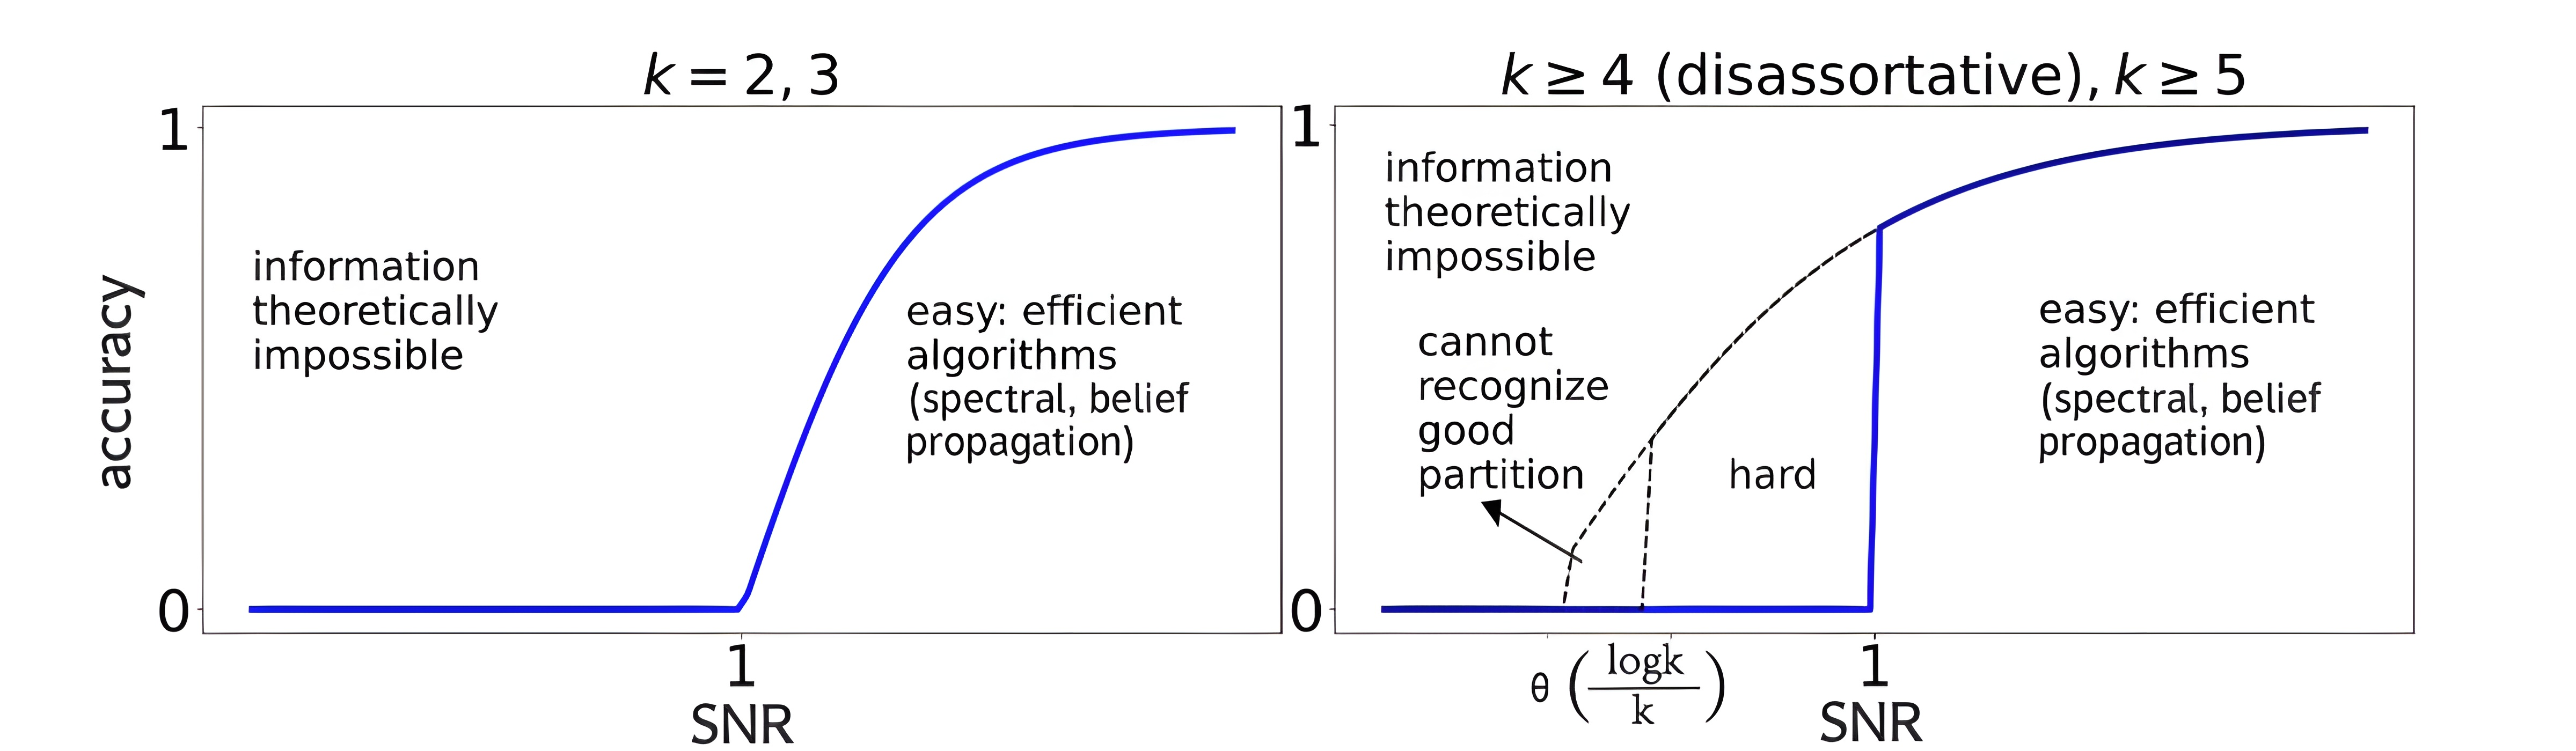
\includegraphics[width=1.1\linewidth]{Figures/phase_trans.jpg}
    \caption[Phase Transition for the Kesten-Stigum Bound Conjecture]{Phase transition for the Kesten-Stigum Bound conjecture. There is a remarkable surge at SNR = 1, where the reconstruction problem shifts from being impossible to achieve efficiently to being efficiently solvable. For $k=2$ and $3$, information-theoretic and computational threshold are both at $SNR$ = 1, but for $k\geq5$ on disassortative case, the information-theoretic threshold is $\theta(logk/k)$ while computation threshold is 1 \cite{TheSurvey}.}
    \label{fig:phase_trans}
\end{figure}
The Kesten-Stigum Bound conjecture describes a phrase transition phenomenon (see figure \ref{fig:phase_trans}), where a desired property becomes almost impossible to achieve below a certain threshold but suddenly becomes highly likely to occur once the threshold is exceeded. Prominent examples include the connectivity of Erd\H{o}s-R\'{e}nyi random graph and Shannon's coding theorem \cite{shannon}. Phrase transition phenomenon has played a crucial role in the development of various algorithms, often serving as a guiding principle \cite{TheConjecture}.\\
Spectral algorithms are arguably the most widely used approaches in community detection, mainly due to its efficiency and mathematical elegance \cite{spectral_algo_review}. Belief propagation and standard spectral algorithms, which include those based on adjacency and Laplacian matrices, are both effective for reconstruction when the graph is sufficiently dense and above the Kesten-Stigum (KS) threshold \cite{standard_spec_in_dense}. However, when the graph is sparse, only belief propagation can achieve the KS threshold \cite{firstpaper}, while standard spectral algorithms fail a significant distance from the KS threshold \cite{standard_spec_fail}. To address this issue, a spectral algorithm based on the non-backtracking matrix was introduced in \cite{the_non-backtracking}, which can be viewed as a linearisation of the belief propagation algorithm\cite{as15c}. the non-backtracking matrix-based spectral algorithm  has been proven to succeed down to the KS threshold in both sparse and dense graphs  \cite{blm15}, bridging the gap between spectral methods and statistical inference in terms of effectiveness for community detection. Furthermore, the non-backtracking matrix-based spectral algorithm is considered one of the most efficient and elegant approaches to the community detection problem \cite{the_non-backtracking} \cite{TheConjecture}.\\
This review doesn't encompass the full spectrum of the existing solutions to community detection. Due to the vast amount of literature on this subject, it is challenging to provide an exhaustive account of all the techniques. For a more thorough exploration, I recommend referring to the papers in \cite{TheConjecture} \cite{comm_dete_in_graphs} \cite{userguide} \cite{dallamico:tel-03454227}.

\section{Overview}
The rest of this report is structured as follows:
\begin{itemize}
    \item Chapter \ref{chapter:2}: This chapter focuses on the easy regime, where SNR $>1.$ We first discuss the standard spectral algorithm and its limitations. Then, we present the spectral algorithm based on the non-backtracking matrix and highlight its advantages.
    \item Chapter \ref{chapter:3}: This chapter focuses on the hard regime, where SNR $\leq1$. We introduce the partial seed set setting and propose a greedy recovery algorithm designed for this setting and discuss some improvements concerning the performance and efficiency of this algorithm. We then provide a mathematical analysis of this algorithm and present experimental results for the two-community case.
    \item Chapter \ref{chapter 4}: This chapter investigates the performance of combining the spectral algorithm and our greedy recovery algorithm for the case of two communities and SNR $>1.$ We explore the potential benefits and limitations of this hybrid approach
    \item Chapter \ref{chapter 5}: This chapter generalises our greedy recovery algorithm to the case of five communities.
    \item Chapter \ref{chapter 6}: This chapter summaries the work done in this project, including the main contributions, limitations, and discuss potential future work.
    \item Chapter \ref{chapter 7}: This chapter discusses project management and methodology.
\end{itemize}
\section{Preliminaries}
\begin{definition}[Adjacency matrix]
    Given $G=(V, E),$ the adjacency matrix $\mathbf{A}$ for $G$ is a $n\times n$ matrix such that\begin{equation*}
    \mathbf{A}_{i, j} = 
    \begin{cases} 
    1 & \text{if } \{i, j\}\in E\\
    0 & \text{otherwise}
    \end{cases}
    \end{equation*}
\end{definition}
\begin{definition}[Laplacian matrix]
Given a simple $G=(V, E),$ the Laplacian matrix $\mathbf{L}$ for $G$ is a $n\times n$ matrix such that\begin{equation*}
    \mathbf{L}_{i, j} = 
    \begin{cases} 
    dge(v_i) & \text{if}~i=j\\
    -1 & \text{if}~i\neq j~\text{and}~\{i, j\}\in E\\
    0 & \text{otherwise}
    \end{cases}
    \end{equation*}
Equivalently, $\mathbf{L}=\mathbf{D}-\mathbf{A},$ where $\mathbf{A}$ is the adjacency matrix and $\mathbf{D}$ is the degree matrix (a diagonal matrix with $\mathbf{D}_{i, i}=deg(i)$).
\end{definition}
\begin{definition}[Non-backtracking matrix]\label{def: non_backtracking}
Given a directed $G=(V, E),$ the non-backtracking matrix $\mathbf{B}$ for $G$ is a $|E|\times |E|$ matrix such that\begin{equation*}
     \mathbf{B}_{(u,v)(\ell,k)} = 
    \begin{cases} 
    1 &~\text{if}~v = \ell~\text{and}~u \neq k \\
    0 &~\text{otherwise}
    \end{cases}
\end{equation*}
\end{definition}
\begin{remark}
This matrix corresponds to a non-backtracking walk, which is a walk that does not repeat a vertex within 2 steps. For example, $u\to v\to w$ is a valid non-backtracking walk, but $u\to v\to u$ is not.
\begin{center}
\begin{tikzpicture}[>=Stealth,shorten >=2pt,node distance=3cm,on grid,auto] 
   \node[circle, draw, minimum size=3em] (u) {\(u\)};
   \node[circle, draw, minimum size=3em] (v) [right=of u] {\(v\)};
   \node[circle, draw, minimum size=3em] (w) [right=of v] {\(w\)};

   \path[->]
    (u) edge node {} (v)
    (v) edge node {} (w);

   \path[->]
    (v) edge [bend right, red, dashed] node {} (u);
\end{tikzpicture}
\end{center}
\end{remark}
\begin{example}
Given the following graph,
\begin{center}
\begin{tikzpicture}[>=Stealth,shorten >=2pt,node distance=3cm,on grid,auto] 
   \node[circle, draw, minimum size=3em] (1) {\(1\)};
   \node[circle, draw, minimum size=3em] (2) [above right=of 1] {\(2\)};
   \node[circle, draw, minimum size=3em] (3) [below right=of 2] {\(3\)};
   \node[circle, draw, minimum size=3em] (4) [below right=of 1] {\(4\)};
   
   \path[->]
    (1) edge[bend left] node[midway, left] {\(e_1\)} (4)
    (4) edge[bend left] node[midway, left] {\(e_2\)} (1)
    (4) edge node[midway, below] {\(e_3\)} (3)
    (3) edge node[midway, right] {\(e_4\)} (2)
    (2) edge node[midway, above] {\(e_5\)} (1);
\end{tikzpicture}
\end{center}
its corresponding non-backtracking matrix $\mathbf{B}$ is
\begin{equation*}
\mathbf{B}=\begin{blockarray}{cccccc}
e_1 & e_2 & e_3 & e_4 & e_5 \\
\begin{block}{(ccccc)c}
  0 & 0 & 1 & 0 & 0 & e_1 \\
  0 & 0 & 0 & 0 & 0 & e_2 \\
  0 & 0 & 0 & 1 & 0 & e_3 \\
  0 & 0 & 0 & 0 & 1 & e_4 \\
  1 & 0 & 0 & 0 & 0 & e_5 \\
\end{block}
\end{blockarray}
\end{equation*}
\end{example}





